\documentclass[11pt,hidelinks,a4paper]{article}
\usepackage[utf8]{inputenc}
\usepackage{datetime}
\ddmmyyyydate
\usepackage{lastpage}
\usepackage[left=2cm,right=2cm,top=2cm,bottom=2cm]{geometry}
\usepackage{fancyhdr}
\usepackage{hyperref}
\makeatletter
\newcommand\urlfootnote@[1]{\footnote{\url@{#1}}}
\DeclareRobustCommand{\urlfootnote}{\hyper@normalise\urlfootnote@}
\makeatother
\usepackage{amsfonts}
	\pagestyle{fancy}
	\setlength{\headheight}{26pt}
	\fancyhf{}
	\rhead{Page \thepage \, of\, \pageref{LastPage}\\ \today}
	\lhead{Joachim Kønigslieb\\ Figures}
\usepackage{amsmath}
\usepackage{graphicx}
\usepackage{parskip}
\usepackage{siunitx}
\usepackage{calligra}
\DeclareMathAlphabet{\mathcalligra}{T1}{calligra}{m}{n}
\DeclareFontShape{T1}{calligra}{m}{n}{<->s*[2.2]callig15}{}
\newcommand{\scriptr}{\mathcalligra{r}\,}
\newcommand{\boldscriptr}{\pmb{\mathcalligra{r}}\,}
\usepackage{float}
\renewcommand{\d}{\,\mbox{d}}
\sisetup{detect-weight=true, detect-family=true}
\renewcommand\thesubsection{\Alph{subsection}}
\sisetup{inter-unit-product=\ensuremath{{}\cdot{}}}
\sisetup{per-mode=fraction}
\sisetup{group-digits=false}
\newcommand*\colvec[3][]{\begin{pmatrix}\ifx\relax#1\relax\else#1\\\fi#2\\#3\end{pmatrix}}
\DeclareSIUnit\time{t}
\DeclareSIUnit\ton{t}
\DeclareSIUnit\cc{c}
\DeclareSIUnit\lysar{ly}
\DeclareSIUnit\unit{u}
\DeclareSIUnit\bq{Bq}
\DeclareSIUnit\year{y}
\DeclareSIUnit\mev{MeV} 
\DeclareSIUnit\parsec{pc}
\usepackage{pdfpages}
\usepackage{hepnames}
\usepackage{xparse}
\newcommand{\g}{\SI{9.82}{\meter\per\second\squared}}
\newcommand{\e}{\, \mbox{e}}
\newcommand{\eps}{\ensuremath{\SI{8.85e-12}{F\per\meter}}}
\newcommand{\unit}[1]{\hat{\mathbf{{#1}}}}
\newcommand\numberthis{\addtocounter{equation}{1}\tag{\theequation}}
\newcommand{\pfrac}[2]{\frac{\partial}{\partial #2}  \left(#1 \right)}
\newcount\colveccount
\newcommand*\change[1]{
        \global\colveccount#1
        \begin{array}{l}
        \colvecnext
}
\def\colvecnext#1{
        #1
        \global\advance\colveccount-1
        \ifnum\colveccount>0
                \\
                \expandafter\colvecnext
        \else
                \end{array}
        \fi
}
\renewcommand{\L}{\mathcal{L}}
\renewcommand{\bf}[1]{\mathbf{#1}}
\usepackage{braket}
\usepackage{rotating}
\begin{document}
\begin{figure}[H]
	\centering
	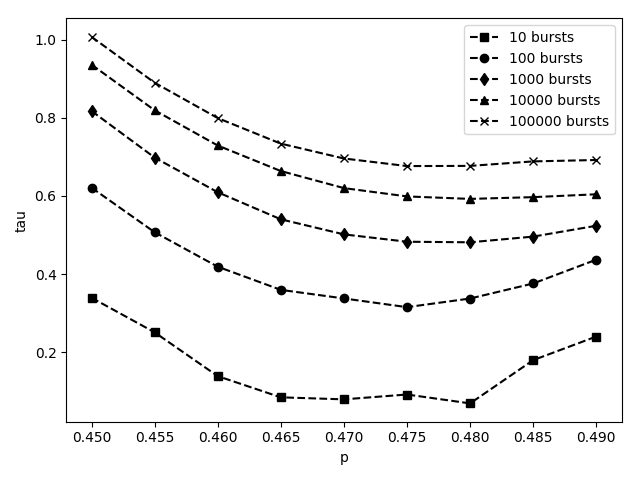
\includegraphics[width=0.80\linewidth]{../tau.png}
	\caption{Fits for $\tau$ with various number of bursts. For each simulation at some $(p,N)$ we simulate 10000 clusters, except at $N=100000$ where we only simulate 1000 clusters.}
\end{figure}
\begin{figure}[H]
	\centering
	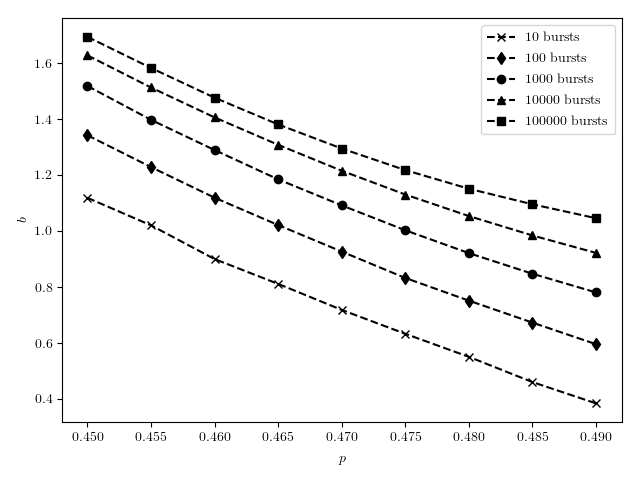
\includegraphics[width=0.80\linewidth]{../bvalue.png}
	\caption{Fits for $b$ with various number of bursts. For each simulation at some $(p,N)$ we simulate 10000 clusters, except at $N=100000$ where we only simulate 1000 clusters.}
\end{figure}
\newpage
\begin{figure}[H]
	\centering
	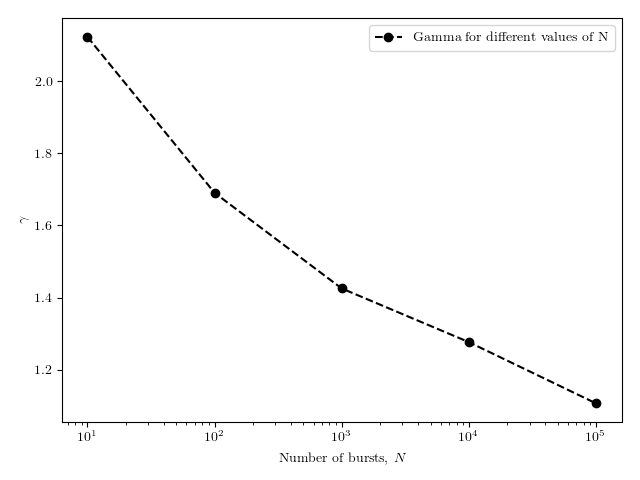
\includegraphics[width=0.80\linewidth]{../gamma.png}
	\caption{Fits for $\gamma$ with various number of bursts. For each simulation at some $(p,N)$ we simulate 10000 clusters, except at $N=100000$ where we only simulate 1000 clusters.}
\end{figure}
\begin{figure}[H]
	\centering
	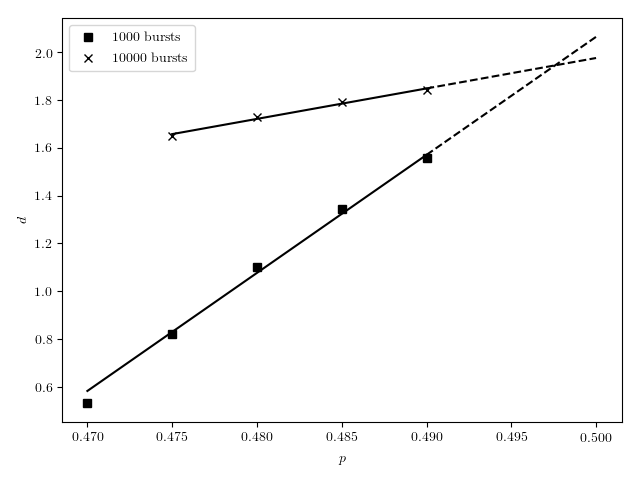
\includegraphics[width=0.80\linewidth]{../fracdim.png}
	\caption{Fits for fractal dimension $d$ with various number of bursts. For each simulation at some $(p,N)$ we simulate 10000 clusters. For the fractal dimensions, only $N={1000,10000}$ are used. For smaller N the results are nonsensical, and for bigger $N$ I run out of harddrive space. }
\end{figure}
\begin{figure}[H]
	\centering
	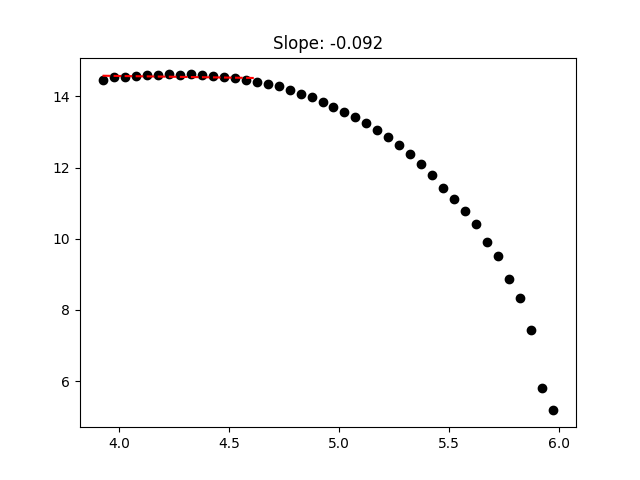
\includegraphics[width=0.8\linewidth]{{../p0.475n100fracdim}.png}
	\caption{Fractal dimension fit for $p=0.475$, $N=100$ bursts. Does not make sense for low $p$ and low $N$. Statistics are gathered over 10,000 clusters of $N$ bursts.}
\end{figure}
\begin{figure}[H]
	\centering
	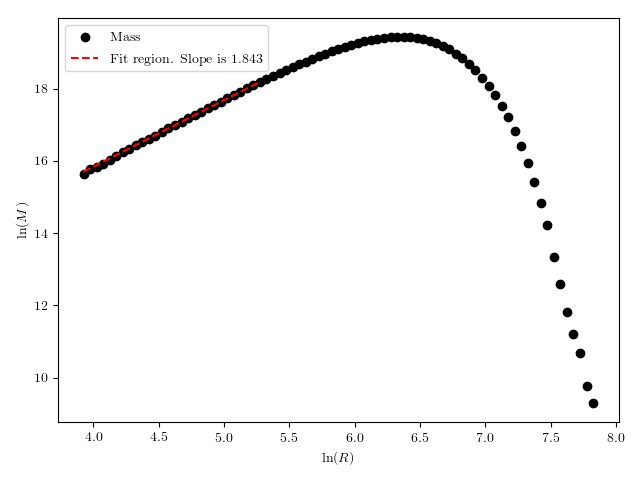
\includegraphics[width=0.8\linewidth]{{../p0.49n10000fracdim}.png}
	\caption{Fractal dimension fit for $p=0.49$, $N=10000$ bursts. It works here! Statistics are gathered over 10,000 clusters of $N$ bursts.}
\end{figure}
\newpage
\begin{figure}[H]
	\centering
	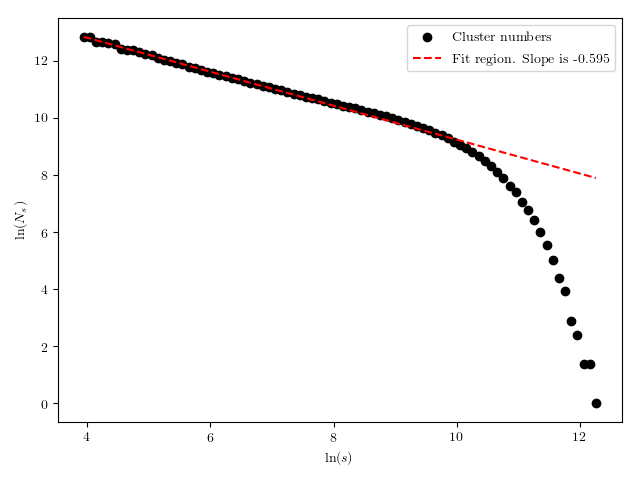
\includegraphics[width=0.8\linewidth]{{../p0.49n10000tau}.png}
	\caption{$p=0.49$, $N=10000$. Fit for $\tau$. This seems to work fine at pretty much all scales. Statistics are gathered over 10,000 clusters of $N$ bursts.}
\end{figure}
\begin{figure}[H]
	\centering
	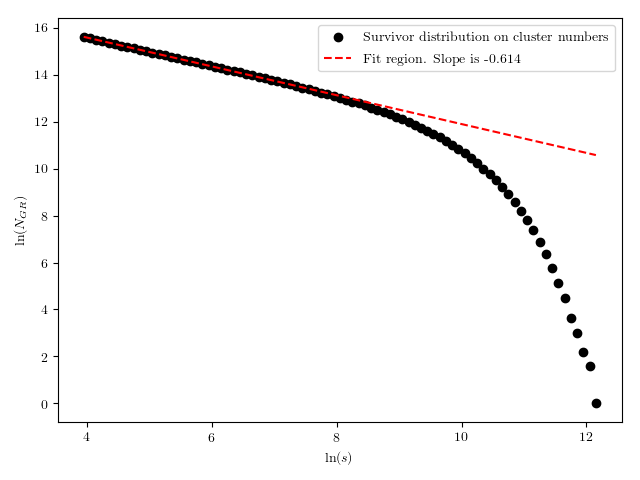
\includegraphics[width=0.8\linewidth]{{../p0.49n10000survivor}.png}
	\caption{$p=0.49$, $N=10000$. Fit on survivor distribution. We can sale this to match Gutenberg-Ricther $b$ value. Note, $\tau$ and $b$ seem to converge to the same value close to percolation threshold but not away from it. Again, 10,000 clusters of $N$ bursts.}
\end{figure}
\newpage
\begin{figure}[H]
	\centering
	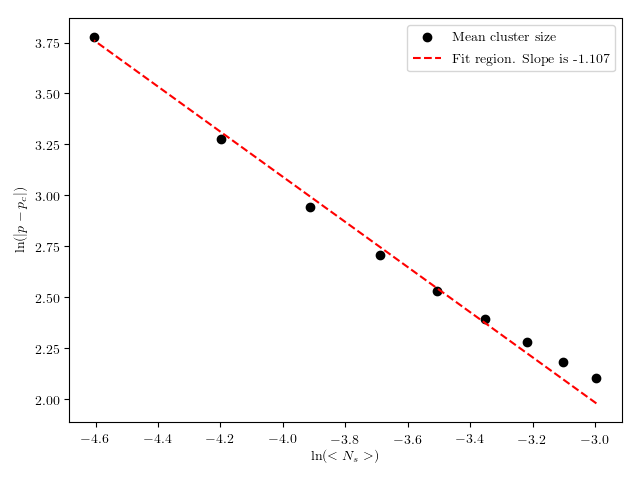
\includegraphics[width=0.8\linewidth]{{../n100000gamma}.png}
	\caption{$p=0.49$, $N=100000$. Here we plot the avergage cluster size for different values of $p-p_c$ and recover the slope on log-log paper. Note we statistics on 1,000 clusters of this bigger $N$ family.}
\end{figure}
\end{document}
